\section{Introduction}

\begin{frame}
	\frametitle{What is ADS?}
	\pnote{Introduce yourself!}
	
\end{frame}

\begin{frame}
	\frametitle{Solving puzzles using computers!}
	\pause
	\framesubtitle{XKCD Logic Boat: \url{https://xkcd.com/1134}}
	
	\begin{figure}
		\begin{subfigure}{0.45\textwidth}
			\includegraphics[width=\textwidth]{figures/logic_boat_1.png}
		\end{subfigure}
		\hfill
		\pause
		\begin{subfigure}{0.45\textwidth}
			\includegraphics[width=\textwidth]{figures/logic_boat_2.png}
		\end{subfigure}
		\label{fig:XKCD 1134: Logic boat}
	\end{figure}
\end{frame}

\begin{frame}
	\frametitle{Real-world problems}
	\framesubtitle{Queuing in the supermarket}
	\begin{center}
		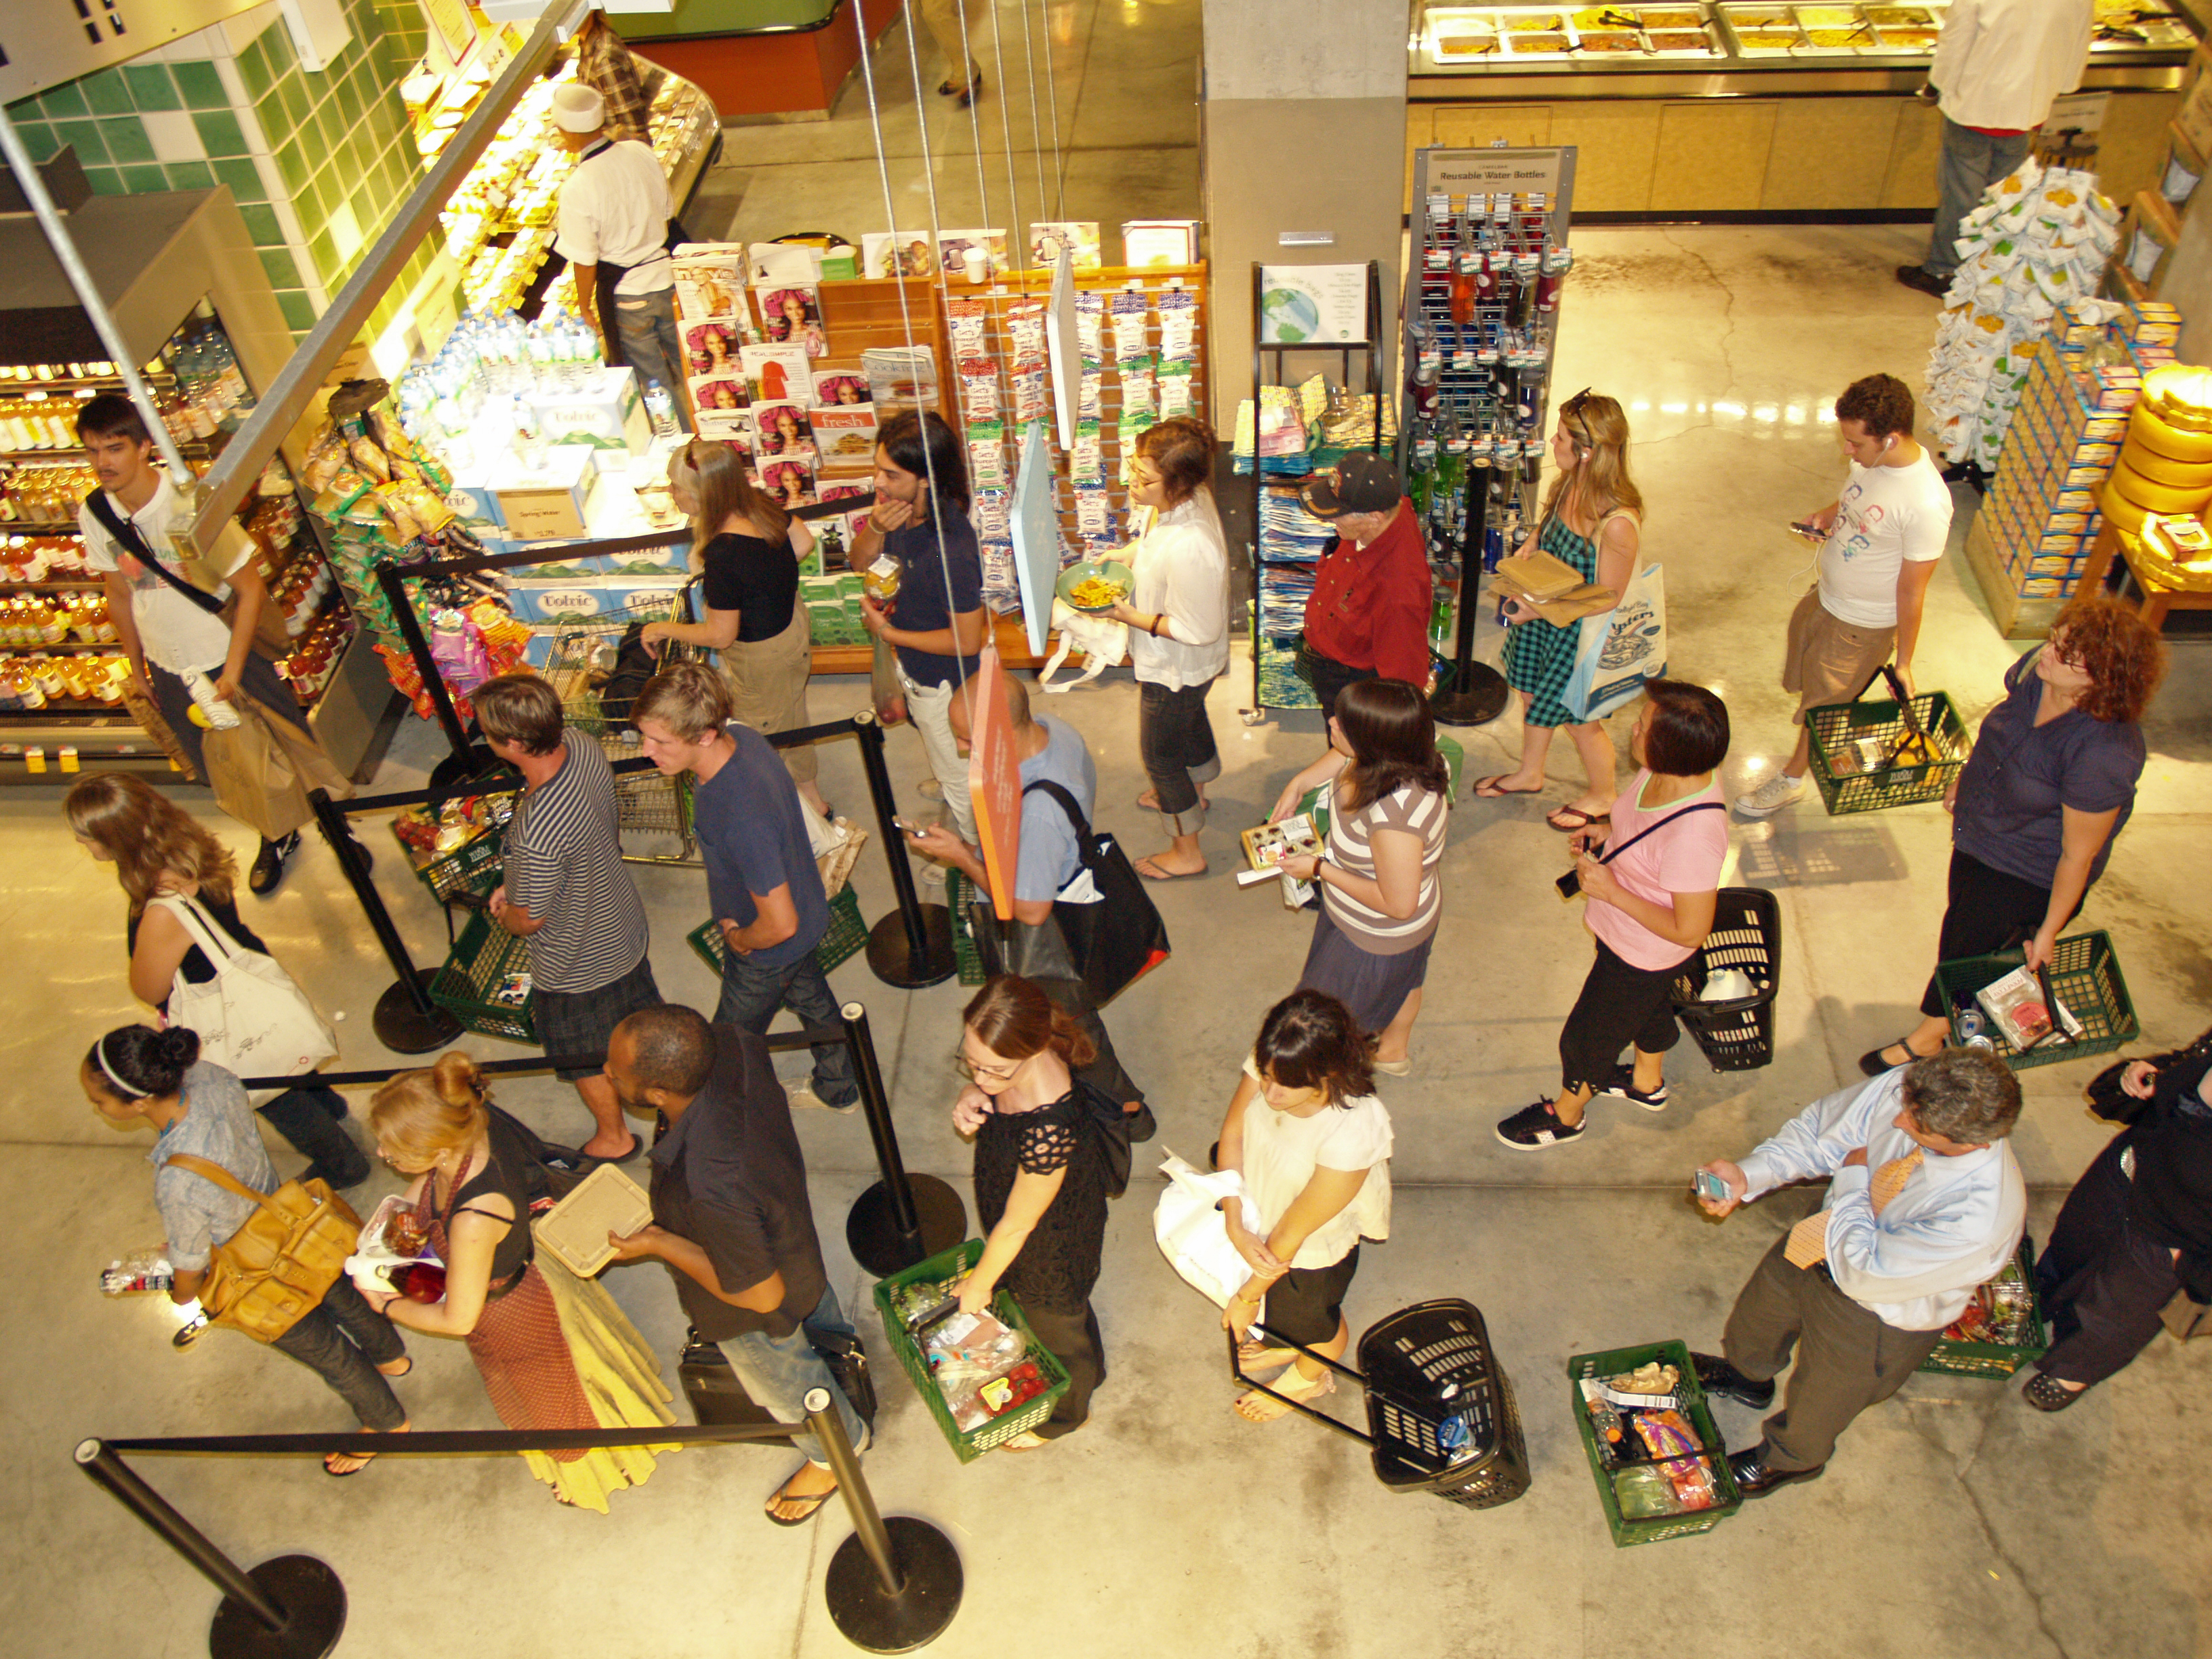
\includegraphics[width=0.6\textwidth]{figures/supermarket.jpg}\\
		\hspace*{15pt}\hbox{\scriptsize Image By:\thinspace{\itshape David Shankbone}}
		%https://commons.wikimedia.org/wiki/File:Waiting_in_line_at_a_food_store.JPG
	\end{center}
	
\end{frame}

\begin{frame}
	\frametitle{Real-world problems}
	\framesubtitle{Finding your way home}
	\begin{center}
		\includegraphics[width=0.6\textwidth]{figures/navigation.jpg}\\
		\hspace*{15pt}\hbox{\scriptsize Image in public domain}
		% https://pxhere.com/en/photo/952741
	\end{center}

\end{frame}

\begin{frame}
	\frametitle{Real-world problems}
	\framesubtitle{Getting the most out of your holiday}
	\begin{center}
		\includegraphics[width=0.5\textwidth]{figures/holidays.jpg}\\
		\hspace*{15pt}\hbox{\scriptsize Images By:\thinspace{\itshape Stefan Hugtenburg}}
	\end{center}
\end{frame}

\begin{frame}
	\frametitle{How do we solve them?}

	\begin{problemblock}{Some real-world problem}
		Given some real-world problem with many bits and pieces of information, how do we solve them?
	\end{problemblock}
	\pause
	\begin{answerblock}{Structure them!}
		\begin{enumerate}
			\item Get the right information out of the problem.
				\pause
				\alert<5->{
			\item Get it into the computer.
			\item Apply an \textit{algorithm} to solve the problem.
			}
				\pause
			\item Get the solution out of the computer.
		\end{enumerate}	
	\end{answerblock}
	\pnote{ADS is (mostly) about step 2 and 3!}
\end{frame}

\subsection{Learning Objectives}
\label{sub:learning_objectives}

\begin{frame}
	\frametitle{So what will I teach you then?}
	\begin{columns}[t]
		\column{0.455\textwidth}
		\begin{block}{Data structures}
			\begin{itemize}
				\item Array-based lists
				\item Linked lists
				\item Queues
				\item Stacks
				\item (Hash)Maps
				\item (Hash)Sets
				\item Trees
				\item Searchtrees
				\item Graphs
			\end{itemize}
		\end{block}	
		\column{0.455\textwidth}
		\pause
		\begin{block}{Algorithms}
			\begin{itemize}
				\item Binary Search
				\item Sorting
				\item Tree traversal
				\item Graph traversal
				\item Shortest paths
			\end{itemize}
		\end{block}	
		\pause
		\begin{alertblock}{All just tools!}
			What I will really teach is you, is how to \textit{solve \st{puzzles} problems}.
		\end{alertblock}	
	\end{columns}
\end{frame}

\begin{frame}
	\frametitle{Rough course-outline}
	\framesubtitle{Know what you are getting into}
	
	\begin{description}[<+->]
		\item[Week 1] Analysing run time and space complexity of algorithms.
		\item[Week 2] Recursive algorithms \& lists
		\item[Week 3] Stacks, Queues \& sorting
		\item[Week 4] Trees \& search trees
		\item[Week 6] Maps \& Graphs
		\item[Week 7] Graph algorithms
		\item[Week 8] P vs NP \& exam prep
	\end{description}
\end{frame}

\begin{frame}
	\frametitle{Short survey time!}
	Just for my curiosity.
	\begin{itemize}
		\item What are you excited about?
		\item Why choose this course?
		\item Programming experience?
	\end{itemize}
	% TODO: [stefan] Find out what survey tool to use. (Fri 04 Jan 2019 04:39:19 PM CET)
\end{frame}
